\section{Calcolo dei pesi, dei carichi e delle spinte}
Al fine di poter effettuare il corretto dimensionamento dell'opera, è necessario considerare i carichi, i pesi e le spinte del sistema.
\begin{figure}[H]
    \centering
    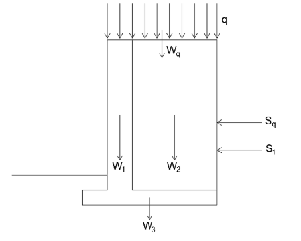
\includegraphics[width=0.5\textwidth]{immagini/pesi_muro.png} \hfill
        \caption{Immagine schematica dei pesi e delle spinte agenti sul muro.}
    \label{figure:pesi_muro}
\end{figure}
\subsection{Calcolo dei pesi}
Il calcolo dei pesi avviene considerando una sezione di muro pari ad 1 metro.\\
\textbf{Muro (mensola verticale)}
\begin{equation*}
    W_1 = \gamma_{cls} \cdot s \cdot H = 25000 \cdot 0.5 \cdot 3 = 37500 \,N/m
\end{equation*}
\textbf{Fondazione (mensola orizzontale)}
\begin{equation*}
    W_2 = \gamma_{cls} \cdot H_f \cdot B = 25000 \cdot 0.5 \cdot 2.65 = 33125 \,N/m
\end{equation*}
\textbf{Terreno }
\begin{equation*}
    W_3 = \gamma_{D} \cdot H \cdot t = 17850 \cdot 3 \cdot 1.75 = 97650 \,N/m
\end{equation*}
\textbf{Carico permanente}
\begin{equation*}
    W_q = q \cdot t = 6000 \cdot 1.75 = 10500 \,N/m
\end{equation*}
\textbf{Peso totale (forza stabilizzante)}
\begin{equation*}
    F_{STAB} = W_1 + W_2 + W_3 + W_q = 37500 + 33125 + 97650 + 10500 = 178775 \,N/m 
\end{equation*}

\subsection{Calcolo delle spinte} 
\textbf{Attiva (teoria di Rankine)}
\begin{equation*}
    S_1 = \frac{1}{2} \cdot K_A \cdot \gamma_D \cdot H^2_t = \frac{1}{2} \cdot 0.33 \cdot 18600 \cdot 3.5^2 = 37975\, N/m
\end{equation*}
\textbf{Carico permanente}
\begin{equation*}
    S_q = q \cdot K_A \cdot H_t = 6000 \cdot 0.33 \cdot 3.5 = 7000 \,N/m
\end{equation*}
\textbf{Spinta totale (forza destabilizzante)}
\begin{equation*}
    F_{DESTAB} = S_1 + S_q = 37975 + 7000 = 44975 \,N/m
\end{equation*}